\providecommand{\dirfunc}[3]{ \frac{ \prod_{#1}^{#2} \g{ #3 } } { \g{ \sum_{#1}^{#2} #3 }}}
\providecommand{\dirnum}[4]{ \frac{\g{ #3 }}{#4} \prod_{#1}^{#2} }
\providecommand{\dirden}[3]{ \g{ \sum_{#1}^{#2} #3 } }

\begin{frame}
\frametitle{Inference}

\begin{itemize}
\item We are interested in posterior distribution
\begin{equation}
p(Z | X, \Theta)
\end{equation}
\pause
\item Here, latent variables are topic assignments $z$ and topics $\theta$.  $X$ is the words (divided into documents), and $\Theta$ are hyperparameters to Dirichlet distributions: $\alpha$ for topic proportion, $\lambda$ for topics.
\begin{equation}
p({\bm z}, {\bm \beta}, {\bm \theta} | {\bm w}, \alpha, \lambda)
\end{equation}
\pause
\begin{align*}
p({\bm w}, {\bm z}, {\bm \theta}, {\bm \beta} & | \alpha, \lambda) = \\
& \prod_{k} p(\beta_k | \lambda) \prod_{d} p(\theta_d | \alpha) \prod_{n}
p(z_{d,n} | \theta_d) p(w_{d,n} | \beta_{z_{d,n}})
\end{align*}
\end{itemize}
\end{frame}



\begin{frame}
\frametitle{Gibbs Sampling}
\begin{itemize}
\item A form of Markov Chain Monte Carlo
\item Chain is a sequence of random variable states
\item Given a state $\{z_1, \dots z_N\}$ given certain technical conditions, drawing $z_k \sim p(z_1, \dots z_{k-1}, z_{k+1}, \dots z_N | X, \Theta)$ for all $k$ (repeatedly) results in a Markov Chain whose stationary distribution \emph{is} the posterior.
\item For notational convenience, call ${\bm z}$ with $z_{d,n}$ removed ${\bm z}_{-d,n}$
\end{itemize}
\end{frame}

\frame{
	\frametitle{Inference}
	\begin{center}
\only<1> {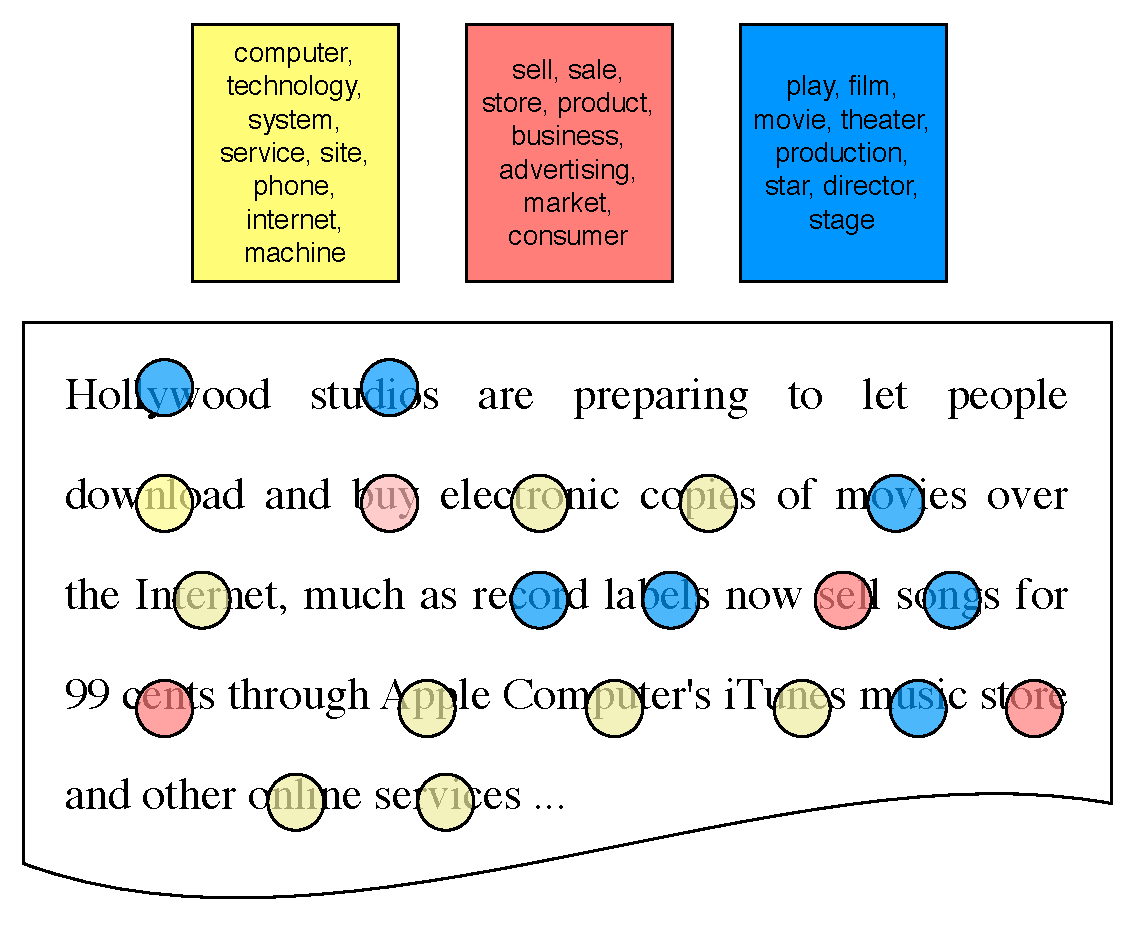
\includegraphics[width=.8\linewidth]{topic_models/inference_3}}
\only<2> {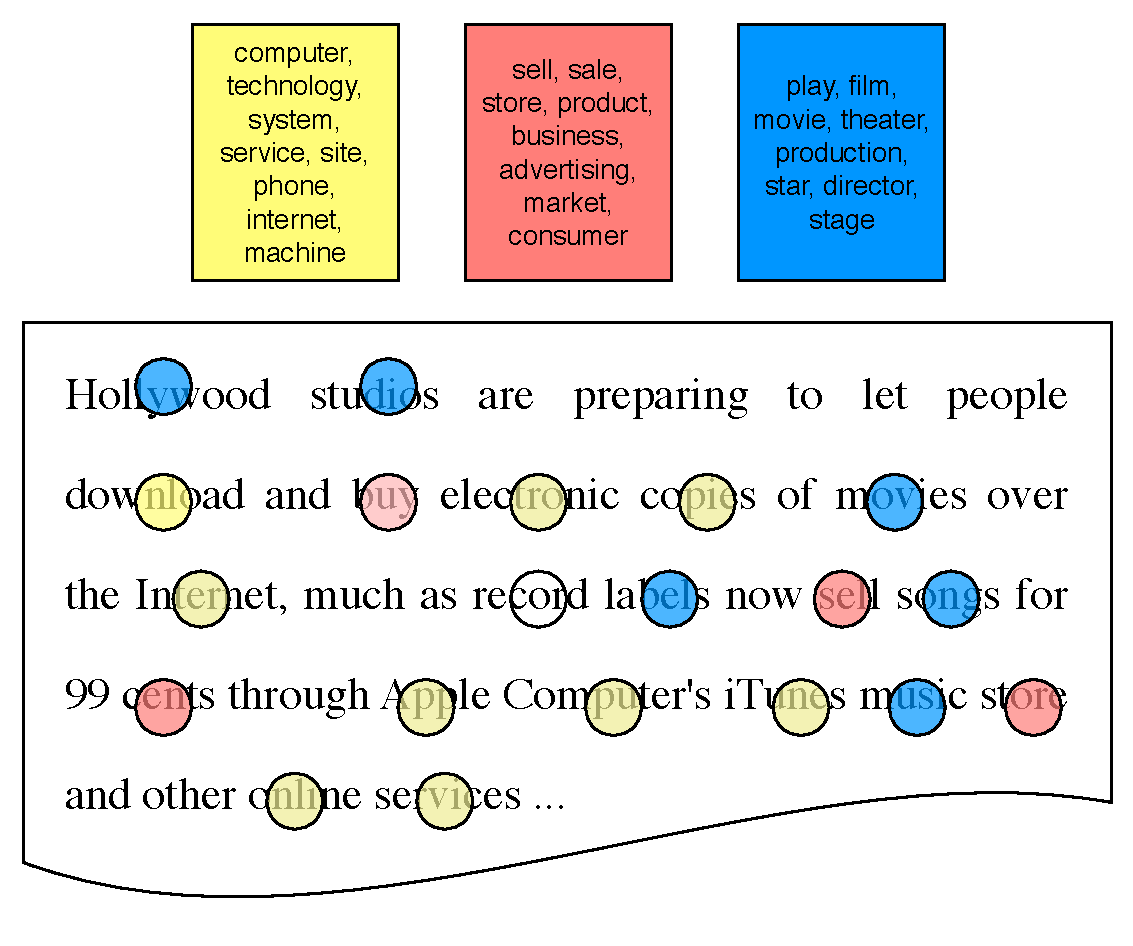
\includegraphics[width=.8\linewidth]{topic_models/inference_4}}
\only<3> {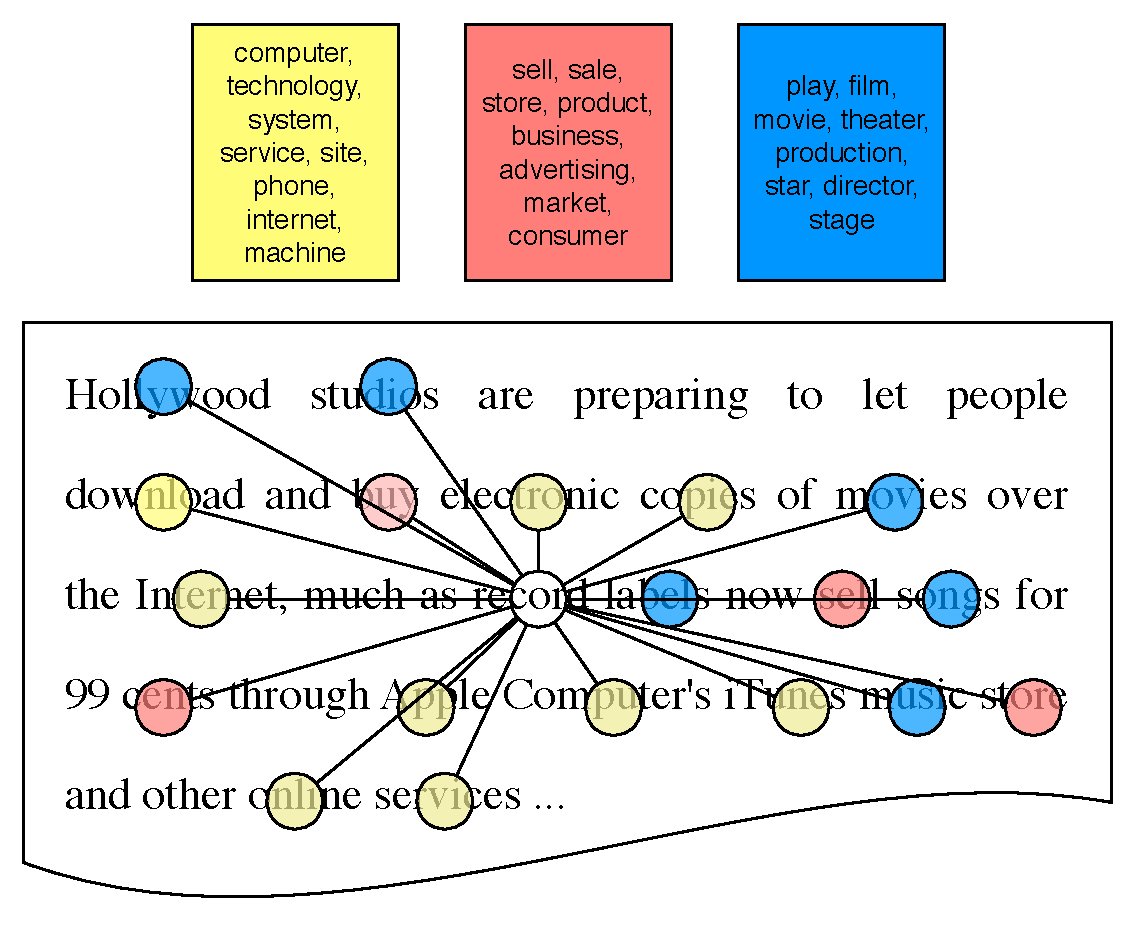
\includegraphics[width=.8\linewidth]{topic_models/inference_5}}
\only<4> {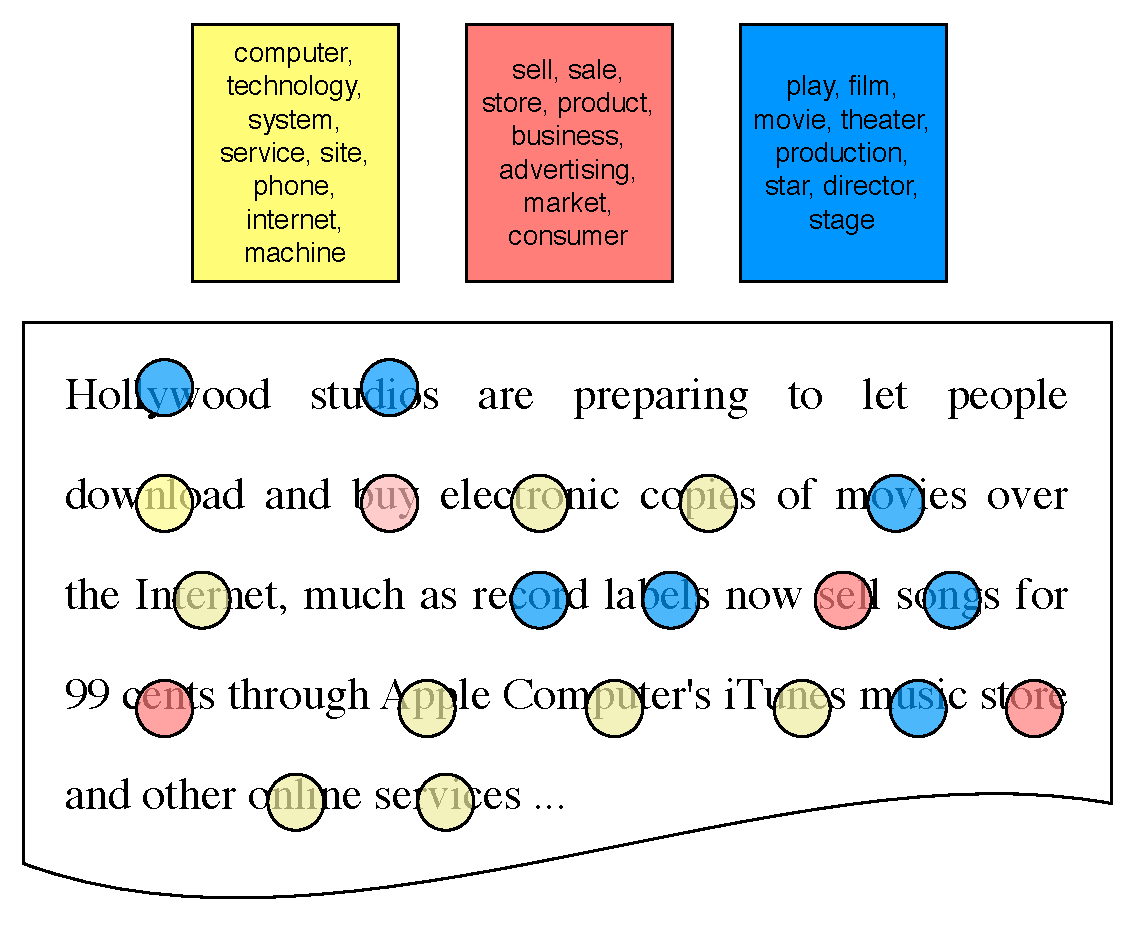
\includegraphics[width=.8\linewidth]{topic_models/inference_3}}
\only<5> {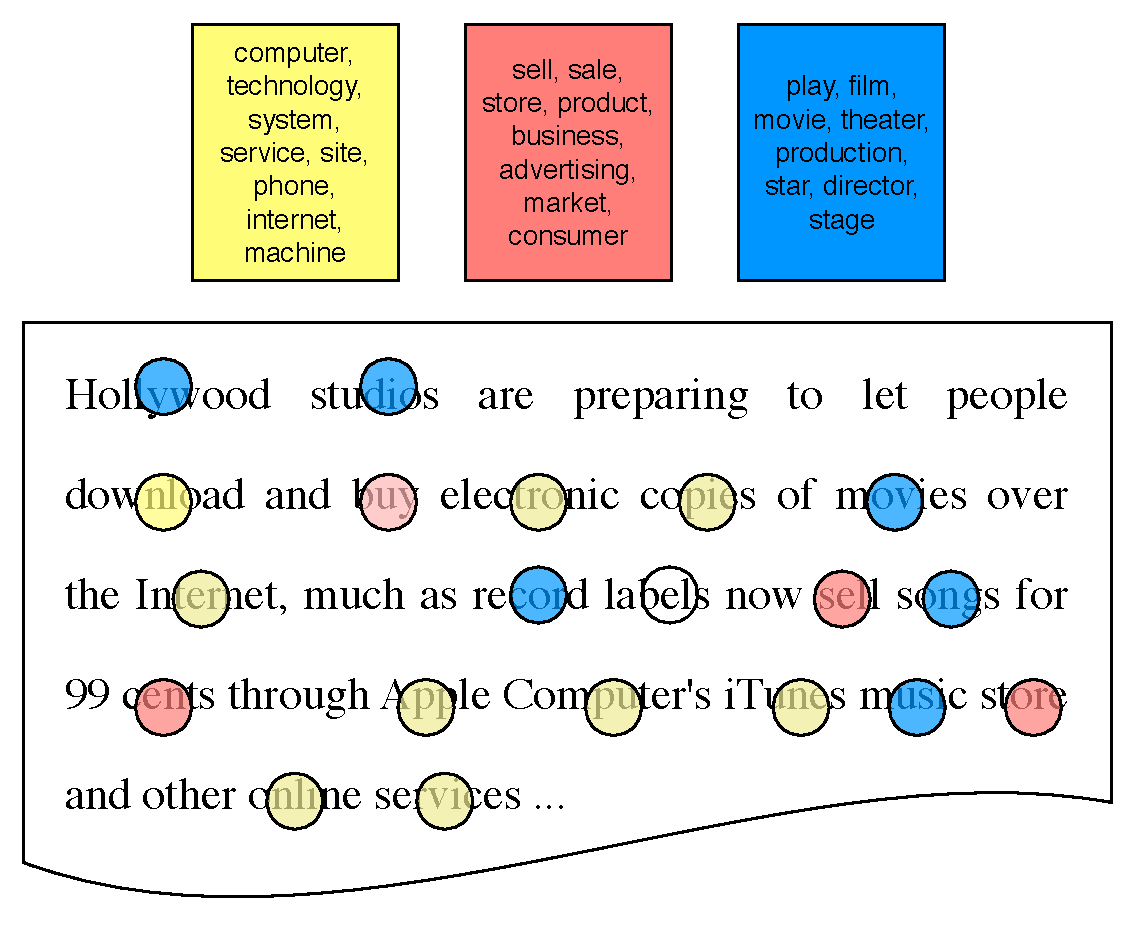
\includegraphics[width=.8\linewidth]{topic_models/inference_6}}
\only<6> {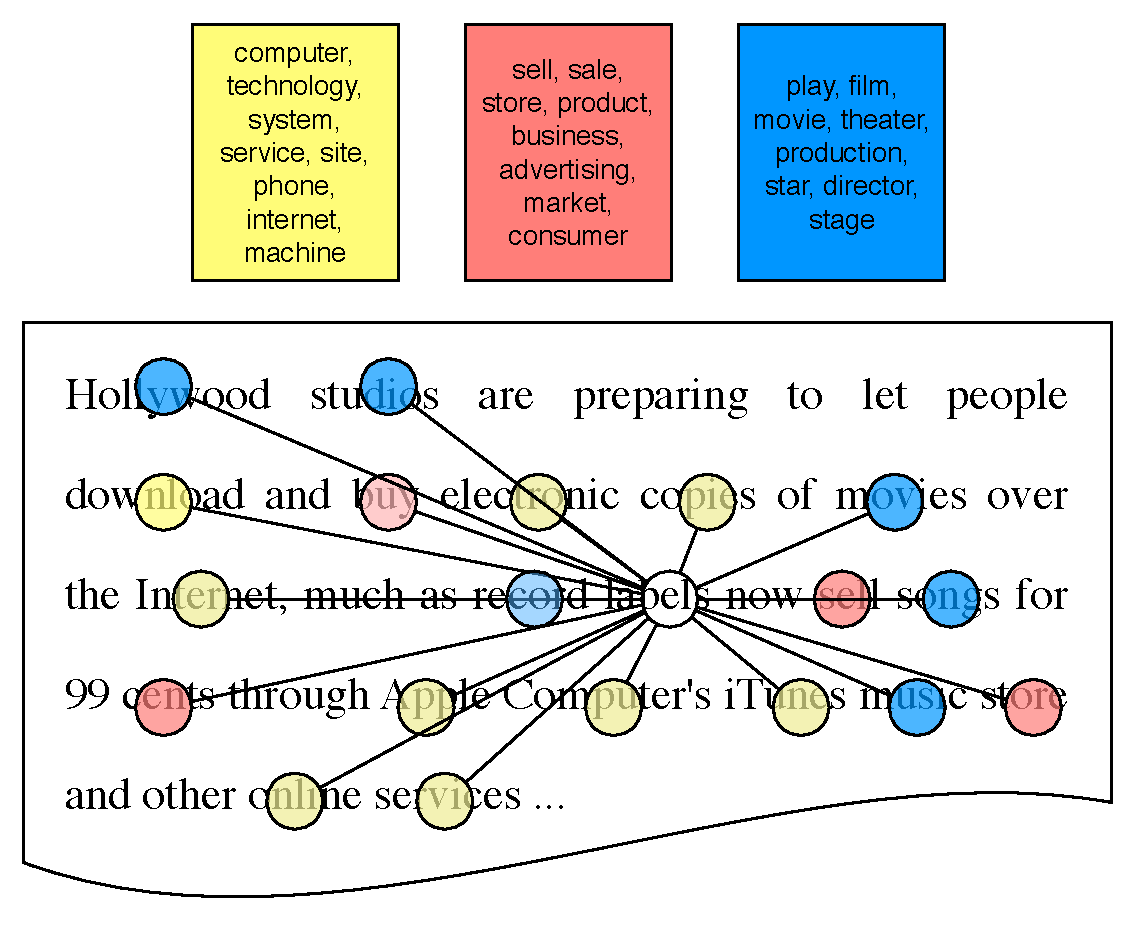
\includegraphics[width=.8\linewidth]{topic_models/inference_7}}
\only<7> {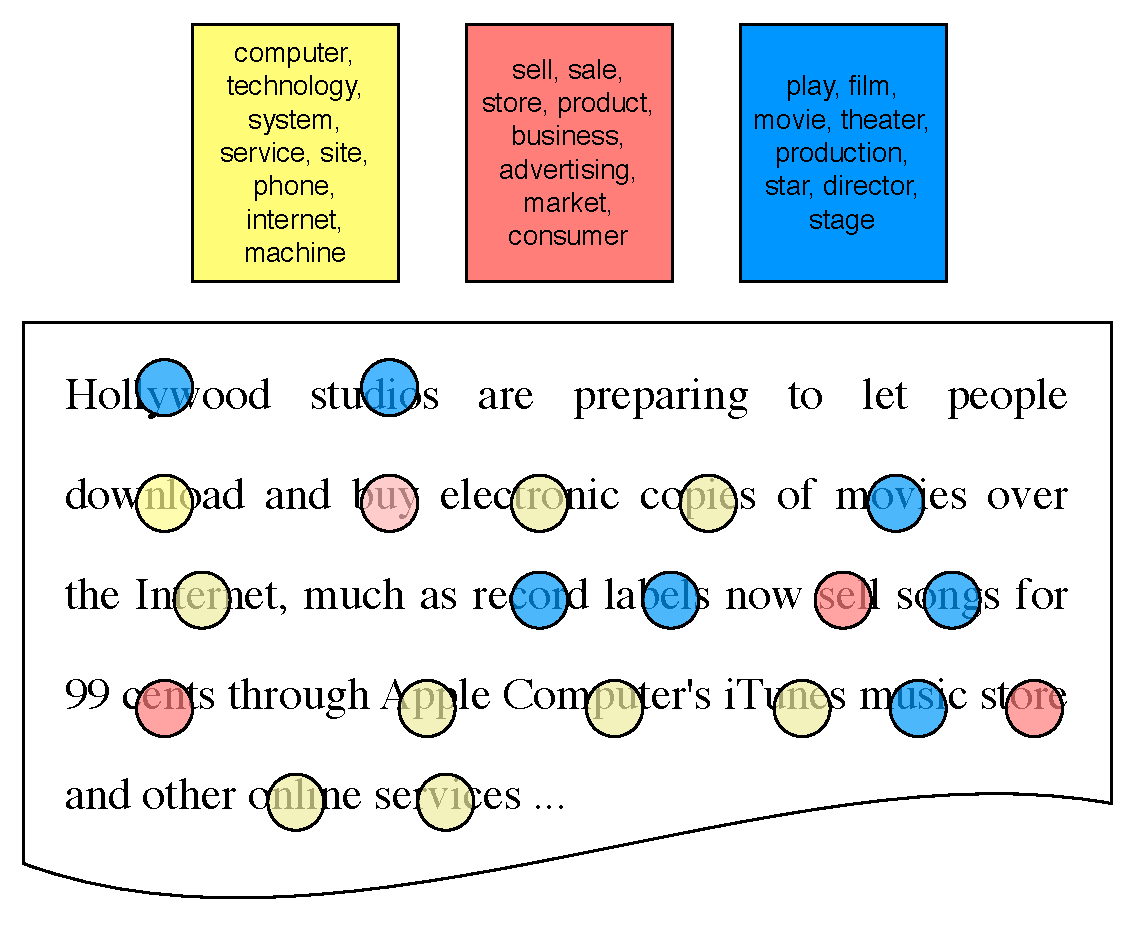
\includegraphics[width=.8\linewidth]{topic_models/inference_3}}
	\end{center}
}


\ifconjugacy

\begin{frame}
\frametitle{Gibbs Sampling}
\begin{itemize}
\item For LDA, we will sample the topic assignments
\item Thus, we want:
\begin{equation*}
p(z_{d,n} = k | {\bm z}_{-d,n}, {\bm w}, \alpha, \lambda) = \frac{ p(z_{d,n} = k, {\bm z}_{-d,n} | {\bm w}, \alpha, \lambda)} { p({\bm z}_{-d,n} | {\bm w},\alpha, \lambda)}
\end{equation*}
\pause
\item The topics and per-document topic proportions are integrated out / marginalized
\item Let $n_{d,i}$ be the number of words taking topic $i$ in document $d$.  Let $v_{k,w}$ be the number of times word $w$ is used in topic $k$.
\end{itemize}


\begin{equation*}
= \frac{ \int_{\theta_d} \left( \prod_{i \not = k} \theta_d^{\alpha_i + n_{d,i} - 1} \right)\theta_d^{\alpha_k + n_{d,i} } d\theta_d \int_{\beta_{k}}    \left( \prod_{i \not = w_{d,n}} \beta_{k,i} ^{ \lambda_i + v_{k,i} - 1} \right) \beta_{k, w_{d,n}}^{\lambda_i + v_{k,i}} d\beta_k } { \int_{\theta_d} \left( \prod_{i} \theta_d^{\alpha_i + n_{d,i} - 1} \right) d\theta_d \int_{\beta_{k}}    \left( \prod_{i} \beta_{k,i} ^{ \lambda_i + v_{k,i} - 1} \right) d\beta_k }
\end{equation*}
\end{frame}

\else

\begin{frame}
\frametitle{Gibbs Sampling}
\begin{itemize}
\item For LDA, we will sample the topic assignments
\item The topics and per-document topic proportions are integrated out / marginalized / Rao-Blackwellized
\item Thus, we want:
\begin{equation*}
p(z_{d,n} = k | {\bm z}_{-d,n}, {\bm w}, \alpha, \lambda) = \frac{n_{d, k} + \alpha_k}{ \sum_{i}^{K} { n_{d,i} + \alpha_i}} \frac{v_{k, w_{d,n}} + \lambda_{w_{d,n}}}{ \sum_{i} { v_{k,i} + \lambda_{i} }}
\end{equation*}
\end{itemize}
\end{frame}

\fi



\ifconjugacy

\begin{frame}
\frametitle{Gibbs Sampling}
\begin{itemize}
\item Integral is normalizer of Dirichlet distribution
\begin{equation*}
\int_{\beta_{k}}    \left( \prod_{i} \beta_{k,i} ^{ \lambda_i + v_{k,i} - 1} \right) d\beta_k = \dirfunc{i}{V}{\beta_i + v_{k,i}}
\end{equation*}
\pause
\item So we can simplify
\end{itemize}
\begin{footnotesize}
\begin{align*}
& \frac{ \int_{\theta_d} \left( \prod_{i \not = k} \theta_d^{\alpha_i + n_{d,i}
      - 1} \right)\theta_d^{\alpha_k + n_{d,i} } d\theta_d \int_{\beta_{k}}
  \left( \prod_{i \not = w_{d,n}} \beta_{k,i} ^{ \lambda_i + v_{k,i} - 1}
  \right) \beta_{k, w_{d,n}}^{\lambda_i + v_{k,i}} d\beta_k } { \int_{\theta_d}
  \left( \prod_{i} \theta_d^{\alpha_i + n_{d,i} - 1} \right) d\theta_d
  \int_{\beta_{k}}    \left( \prod_{i} \beta_{k,i} ^{ \lambda_i + v_{k,i} - 1}
  \right) d\beta_k } = \\
& \frac{
  \dirnum{i \not = k}{K}{\alpha_k + n_{d,k} + 1}{ \g{\sum_{i}^{K} \alpha_i +
      n_{d,i} + 1} } \g{\alpha_k + n_{d,k}}  }
{ \dirfunc{i}{K}{\alpha_i + n_{d,i}} }
% -----------------------------------
\frac{
 \dirnum{i \not = w_{d,n}}{V}{\lambda_{w_{d,n}} + v_{k,w_{d,n}} + 1}{ \g{\sum_{i}^{V} \lambda_i + v_{k,i} + 1} } \g{\lambda_k + v_{k,w_{d,n}}}
}{ \dirfunc{i}{V}{\lambda_i + v_{k,i}} } \\
% -----------------------------------
\end{align*}
\end{footnotesize}
\end{frame}


\begin{frame}

\begin{block}{Gamma Function Identity}
	\begin{equation}
		z = \frac{\Gamma(z + 1)}{\Gamma(z)}
	\end{equation}
\end{block}

\begin{footnotesize}
\begin{align*}
& \frac{
  \dirnum{i \not = k}{K}{\alpha_k + n_{d,k} + 1}{ \g{\sum_{i}^{K} \alpha_i +
      n_{d,i} + 1} } \g{\alpha_k + n_{d,k}}  }
{ \dirfunc{i}{K}{\alpha_i + n_{d,i}} }
% -----------------------------------
\frac{
 \dirnum{i \not = w_{d,n}}{V}{\lambda_{w_{d,n}} + v_{k,w_{d,n}} + 1}{ \g{\sum_{i}^{V} \lambda_i + v_{k,i} + 1} } \g{\lambda_k + v_{k,w_{d,n}}}
}{ \dirfunc{i}{V}{\lambda_i + v_{k,i}} } \\
% -----------------------------------
& = \frac{n_{d, k} + \alpha_k}{ \sum_{i}^{K} { n_{d,i} + \alpha_i}} \frac{v_{k, w_{d,n}} + \lambda_{w_{d,n}}}{ \sum_{i} { v_{k,i} + \lambda_{i} }}
\end{align*}
\end{footnotesize}

\end{frame}
\else
\fi

\begin{frame}{Gibbs Sampling Equation}
  
\begin{equation}
\alert<5>{\frac{\alert<1>{n_{d, k}} +  \alert<3>{\alpha_k}}{ \sum_{i}^{K} { n_{d,i} +\alpha_i}}} \alert<6>{\frac{\alert<2>{v_{k, w_{d,n}}} + \alert<4>{\lambda_{w_{d,n}}}}{ \sum_{i} { v_{k,i} + \lambda_{i} }}}
\end{equation}

\begin{itemize}
  \item \alert<1>{Number of times document $d$ uses topic $k$}
  \item \alert<2>{Number of times topic $k$ uses word type $w_{d,n}$}
  \item \alert<3>{Dirichlet parameter for document to topic
      distribution}
  \item \alert<4>{Dirichlet parameter for topic to word distribution}
  \item \alert<5>{How much this document likes topic $k$}
  \item \alert<6>{How much this topic likes word $w_{d,n}$}
\end{itemize}

\end{frame}

\begin{frame}
  \frametitle{Sample Document}
    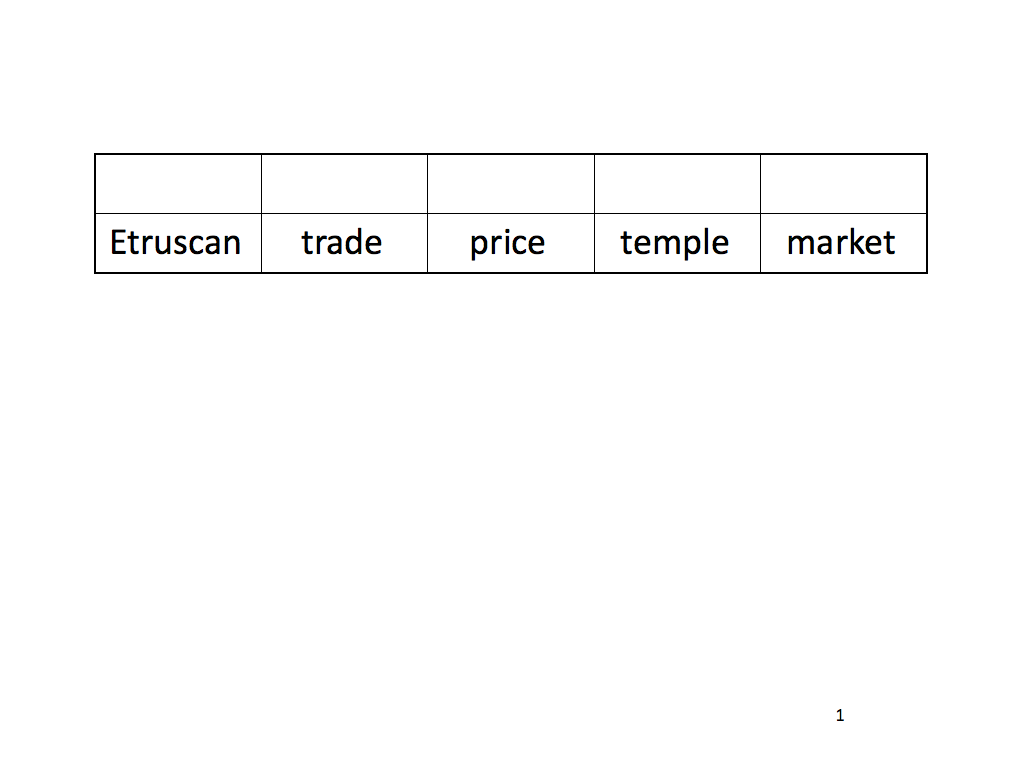
\includegraphics[width=\linewidth]{topic_models/mimno_001}
\end{frame}

\begin{frame}
  \frametitle{Sample Document}
    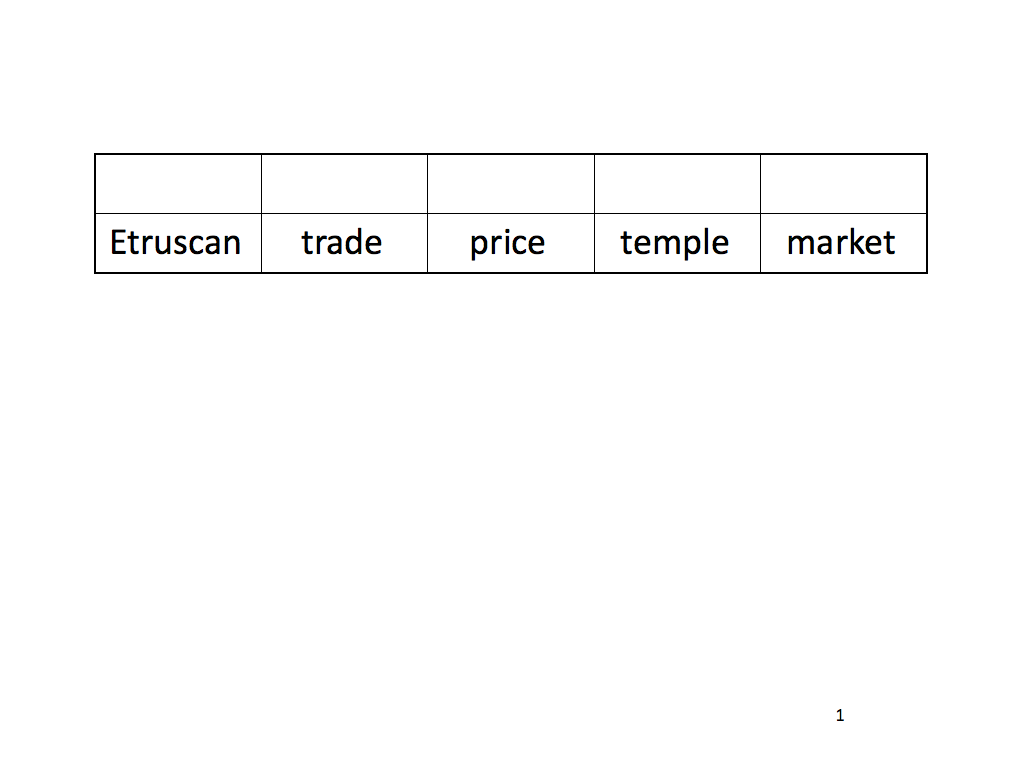
\includegraphics[width=\linewidth]{topic_models/mimno_001}
\end{frame}

\begin{frame}
  \frametitle{Randomly Assign Topics}
    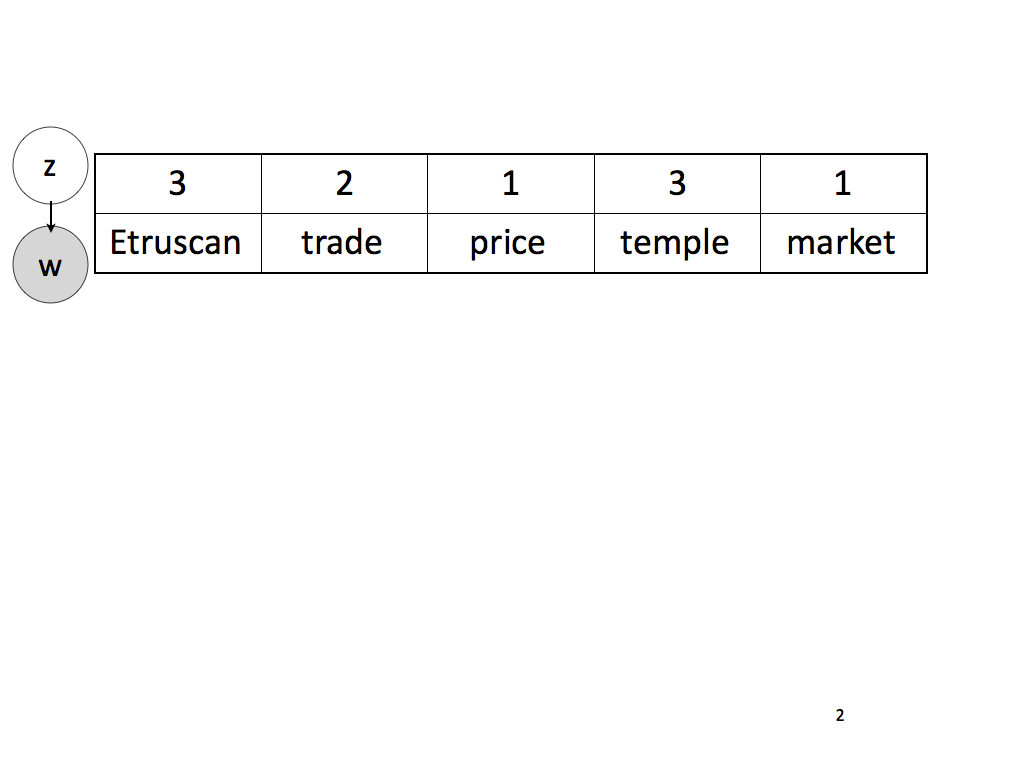
\includegraphics[width=\linewidth]{topic_models/mimno_002}
\end{frame}

\begin{frame}
  \frametitle{Randomly Assign Topics}
    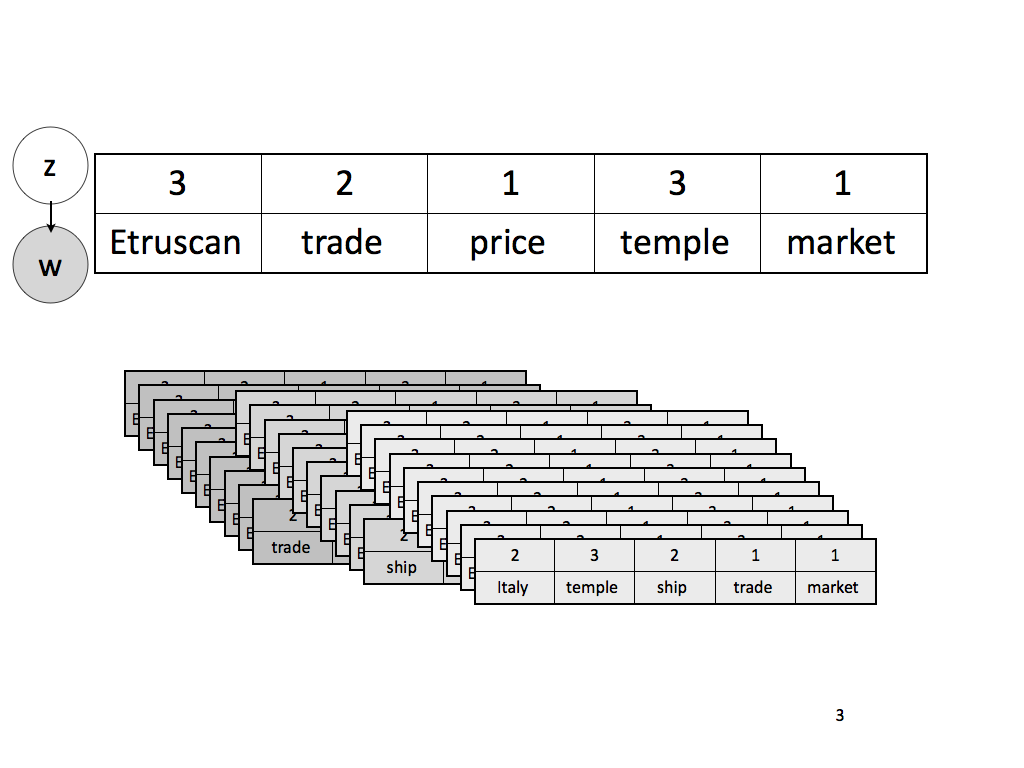
\includegraphics[width=\linewidth]{topic_models/mimno_003}
\end{frame}

\begin{frame}
  \frametitle{Total Topic Counts}
    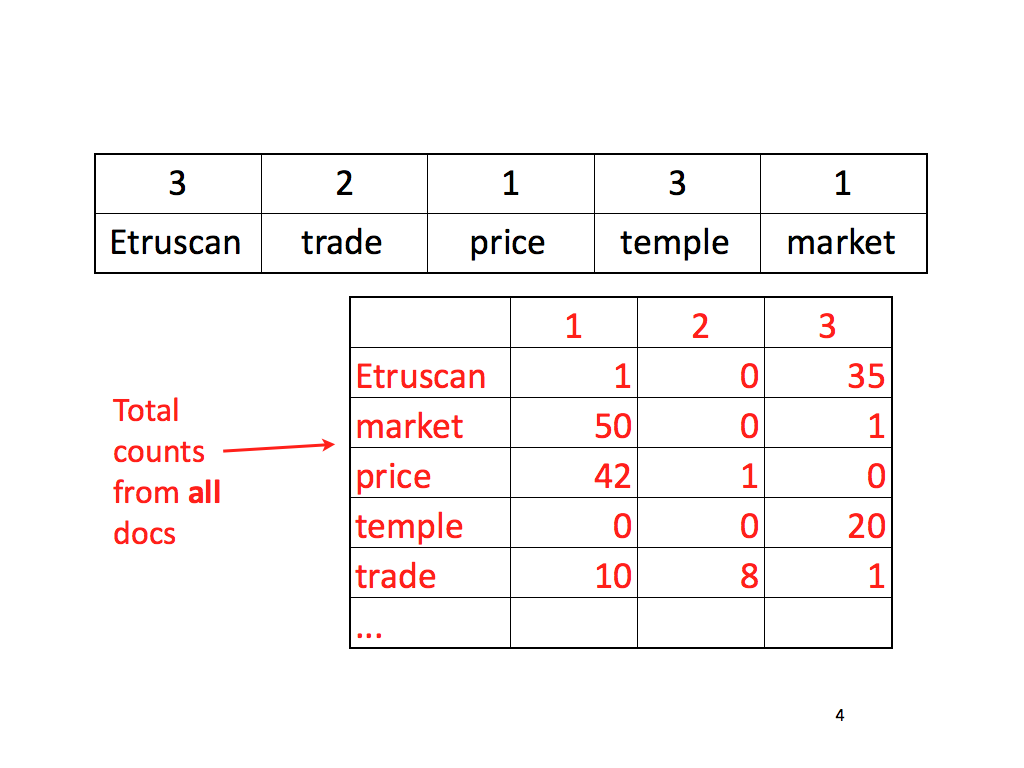
\includegraphics[width=\linewidth]{topic_models/mimno_004}

\pause

\vspace{-4cm}

\begin{block}{Sampling Equation}
	\begin{equation*}
          \frac{n_{d, k} + \alpha_k}{ \sum_{i}^{K} { n_{d,i} + \alpha_i}} \frac{\alert<3>{v_{k, w_{d,n}}} + \lambda_{w_{d,n}}}{ \sum_{i} { \alert<3>{v_{k,i}} + \lambda_{i} }}
	\end{equation*}
\end{block}

\end{frame}


\begin{frame}
  \frametitle{We want to sample this word \dots}
    \only<1>{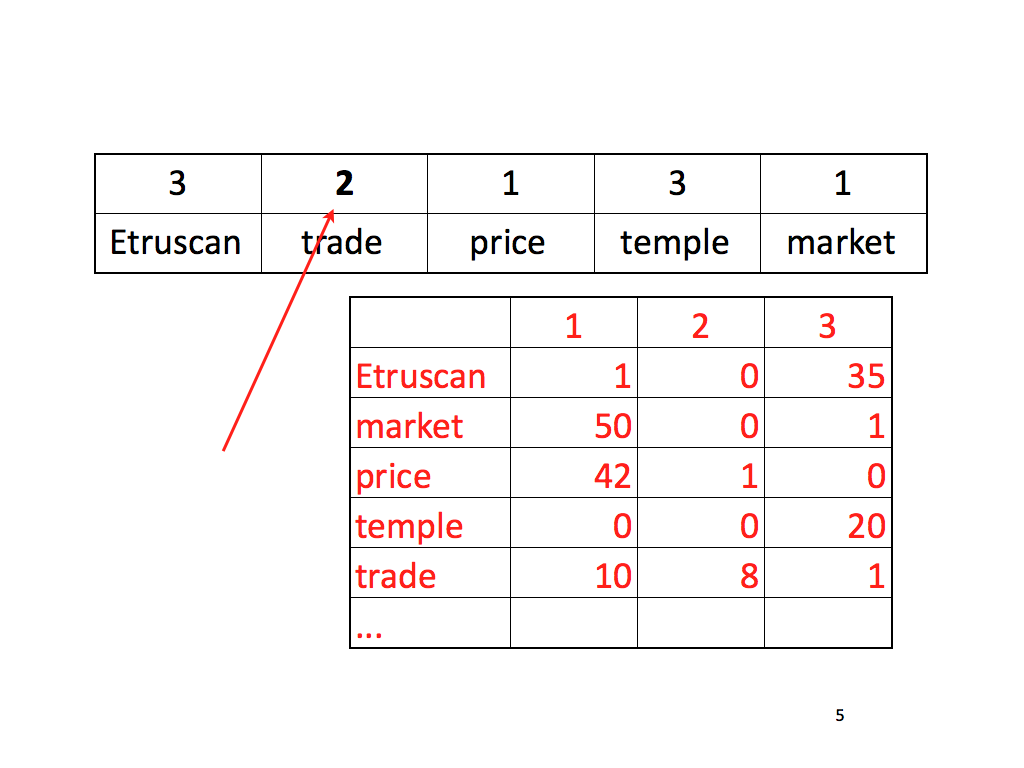
\includegraphics[width=\linewidth]{topic_models/mimno_005}}
    \only<2>{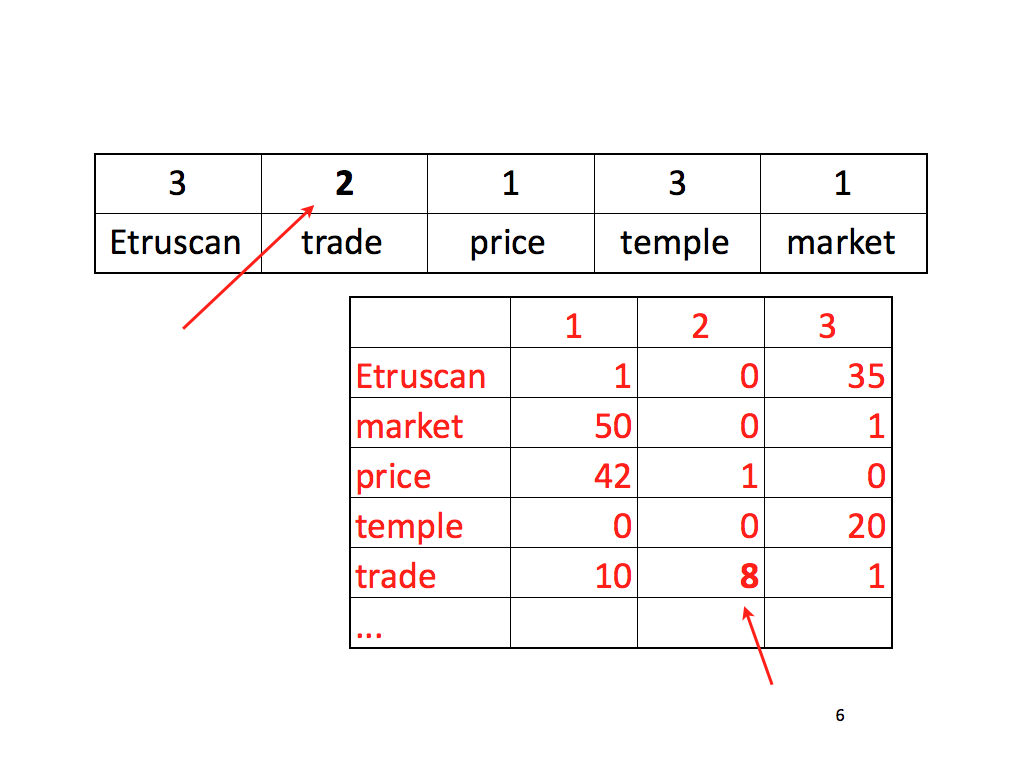
\includegraphics[width=\linewidth]{topic_models/mimno_006}}
\end{frame}

\begin{frame}
  \frametitle{Decrement its count}
    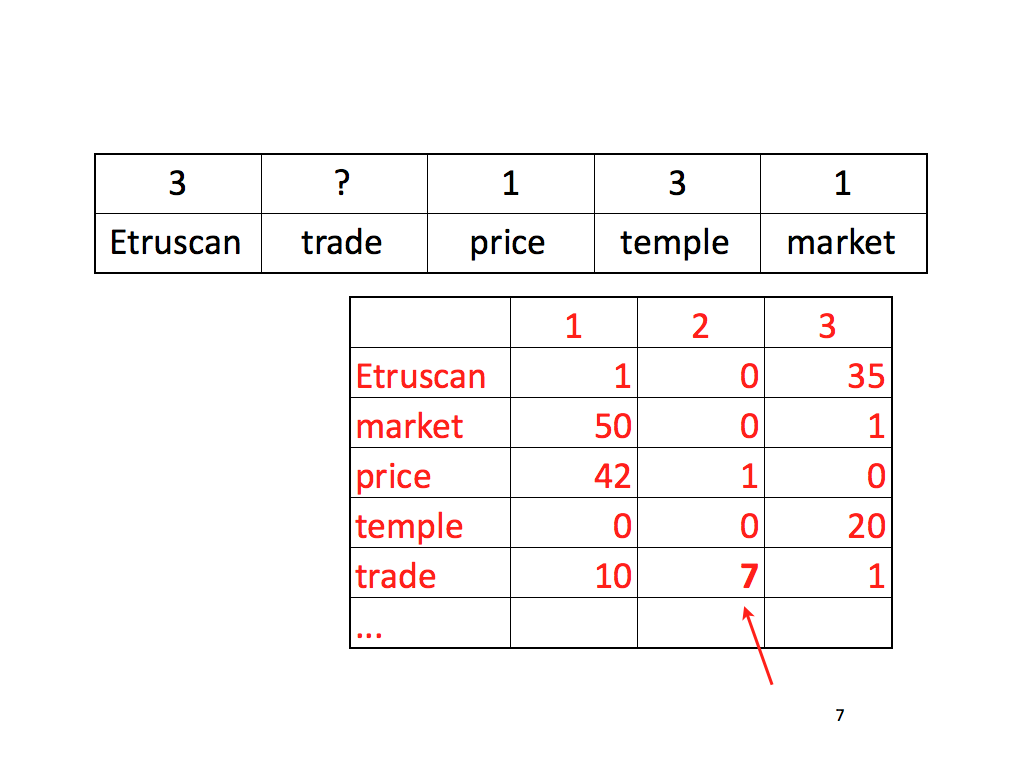
\includegraphics[width=\linewidth]{topic_models/mimno_007}
\end{frame}

\begin{frame}
  \frametitle{What is the conditional distribution for this topic?}
    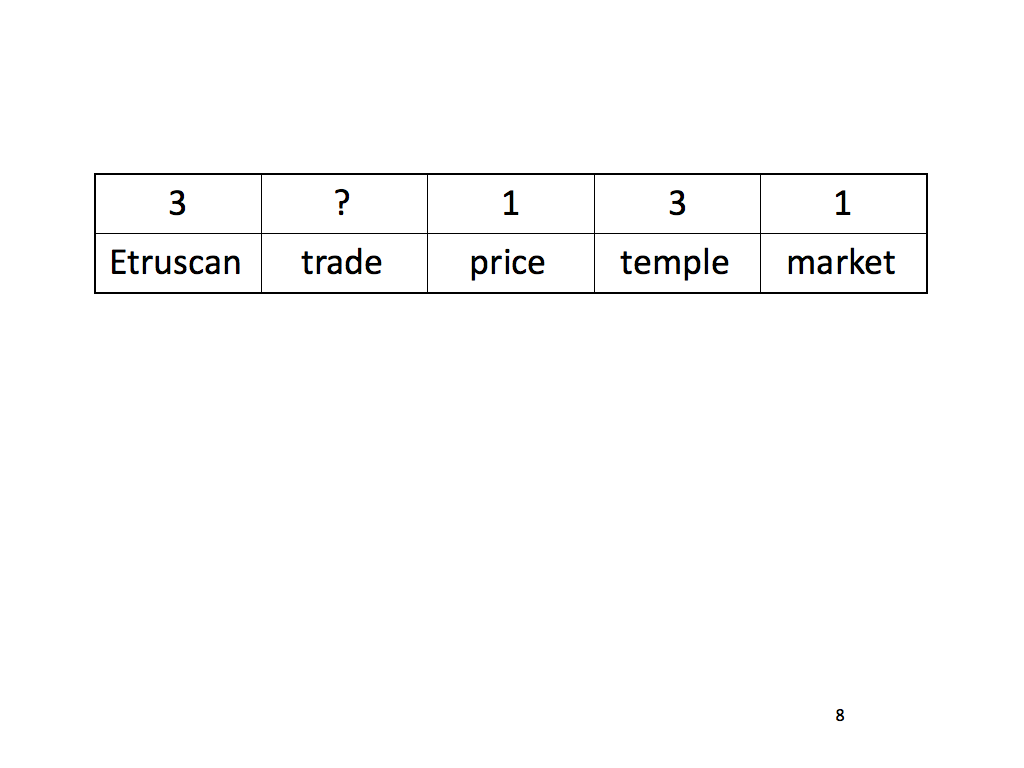
\includegraphics[width=\linewidth]{topic_models/mimno_008}
\end{frame}


\begin{frame}
  \frametitle{Part 1: How much does this document like each topic?}
    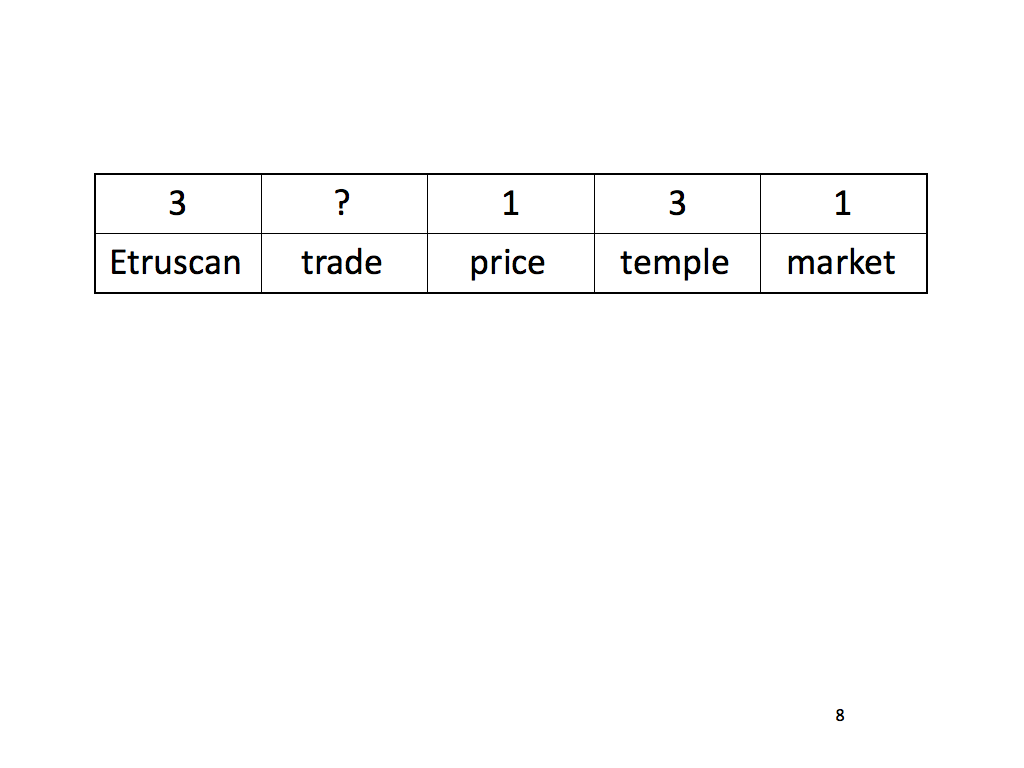
\includegraphics[width=\linewidth]{topic_models/mimno_008}
\end{frame}

\begin{frame}
  \frametitle{Part 1: How much does this document like each topic?}
    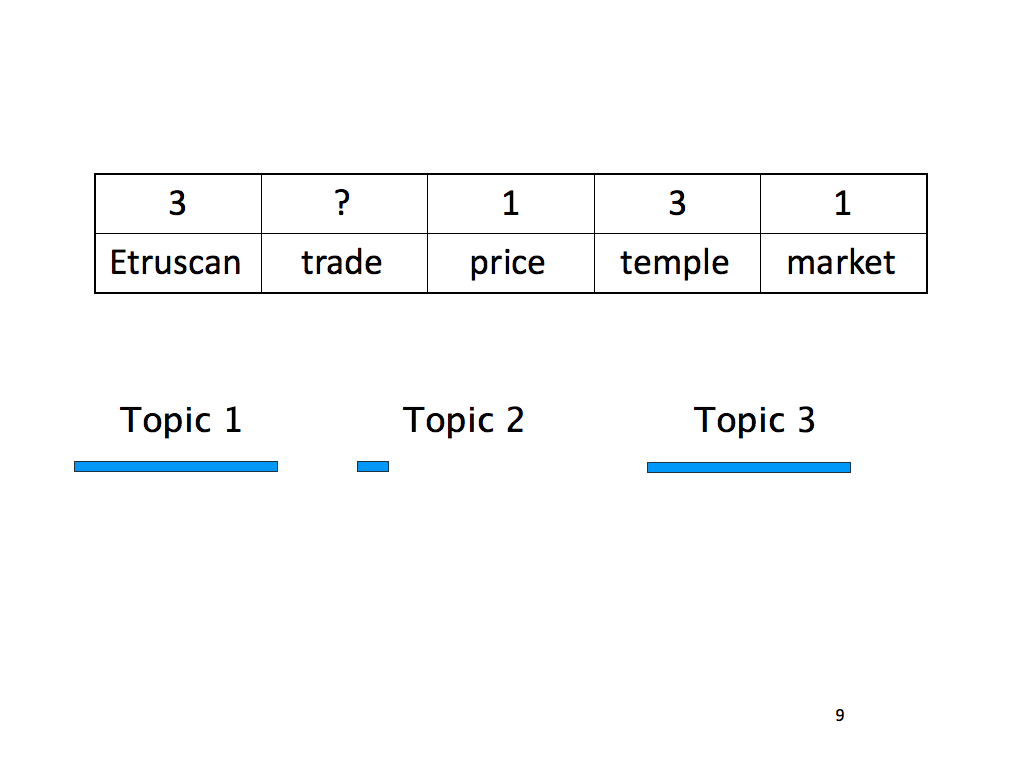
\includegraphics[width=\linewidth]{topic_models/mimno_009}

    \pause
    \vspace{-5cm}
    \begin{block}{Sampling Equation}
	\begin{equation*}
          \frac{\alert<3>{n_{d, k}} + \alpha_k}{ \sum_{i}^{K} { \alert<3>{n_{d,i}} + \alpha_i}} \frac{v_{k, w_{d,n}} + \lambda_{w_{d,n}}}{ \sum_{i} { v_{k,i} + \lambda_{i} }}
	\end{equation*}
     \end{block}


\end{frame}


\begin{frame}
  \frametitle{Part 2: How much does each topic like the word?}
    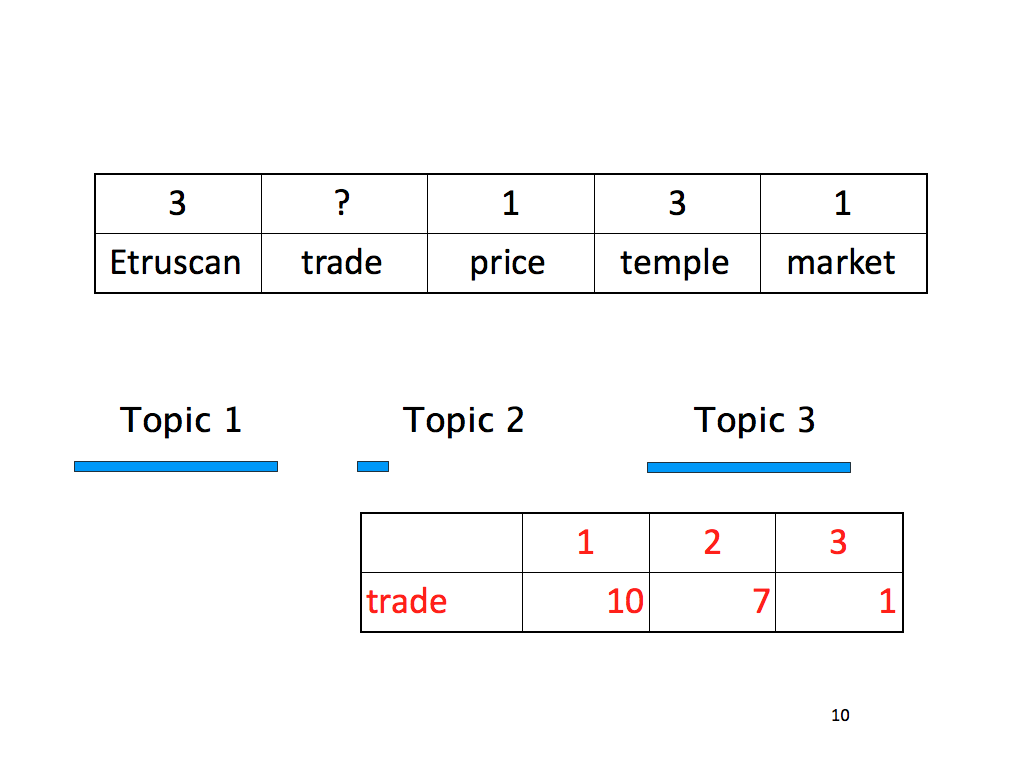
\includegraphics[width=\linewidth]{topic_models/mimno_010}

\pause

\vspace{-4cm}

\begin{block}{Sampling Equation}
	\begin{equation*}
          \frac{n_{d, k} + \alpha_k}{ \sum_{i}^{K} { n_{d,i} + \alpha_i}} \frac{\alert<3>{v_{k, w_{d,n}}} + \lambda_{w_{d,n}}}{ \sum_{i} { \alert<3>{v_{k,i}} + \lambda_{i} }}
	\end{equation*}
\end{block}

\end{frame}


\begin{frame}
  \frametitle{Geometric interpretation}
    \only<1>{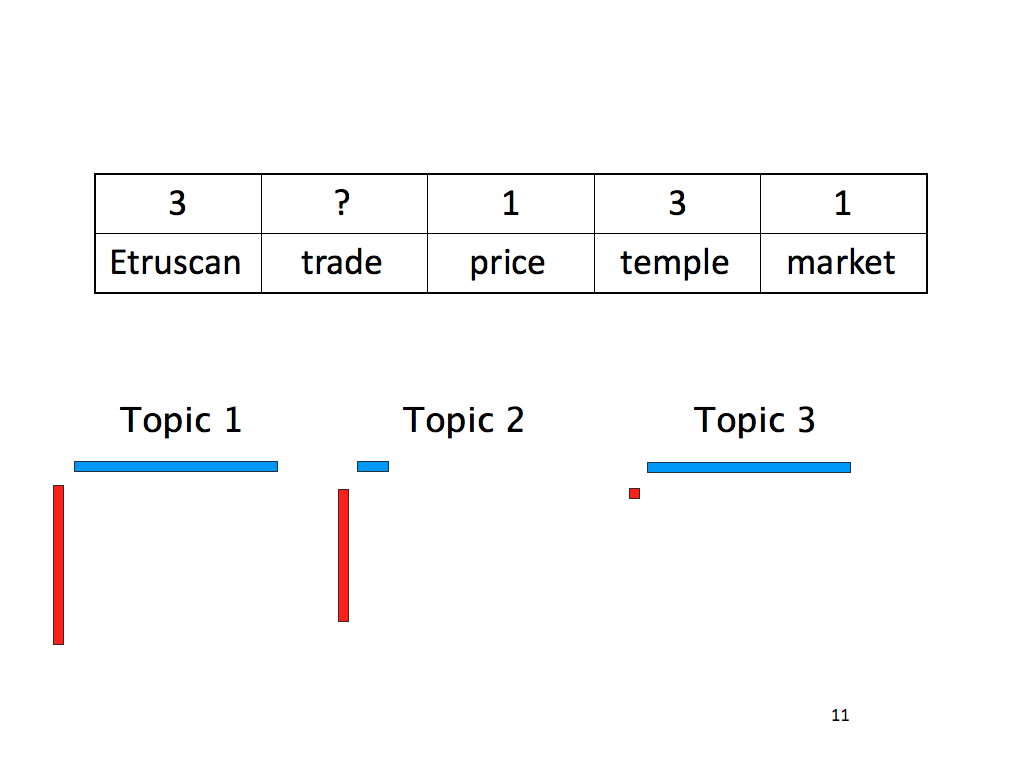
\includegraphics[width=\linewidth]{topic_models/mimno_011}}
    \only<2>{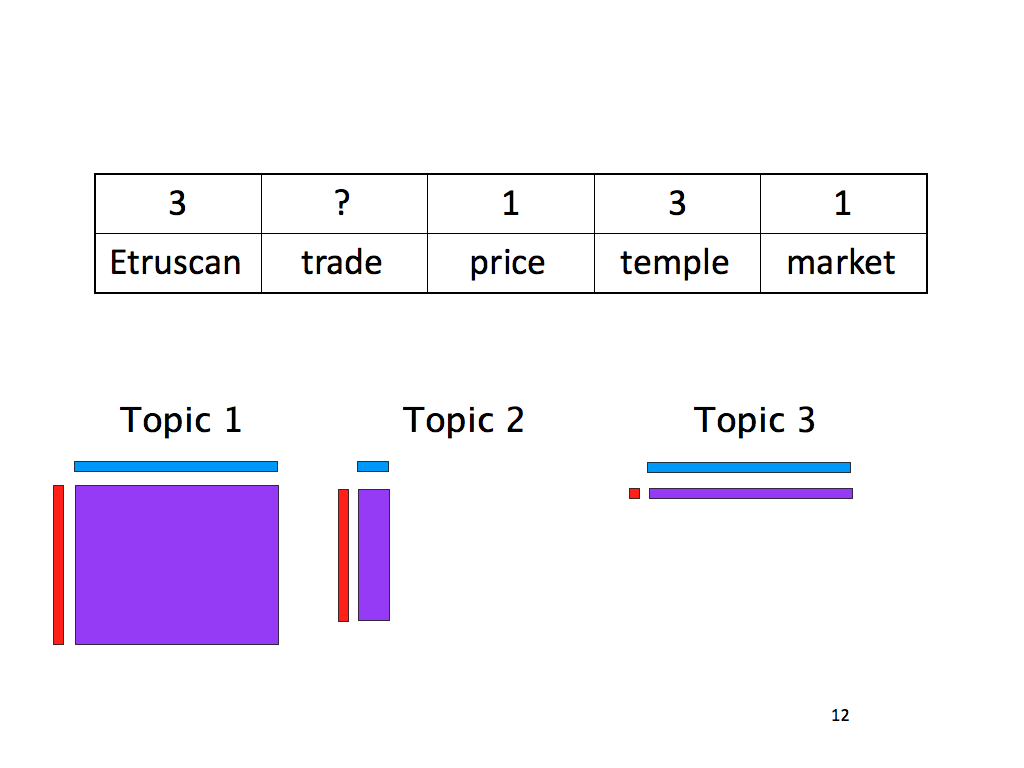
\includegraphics[width=\linewidth]{topic_models/mimno_012}}
    \only<3>{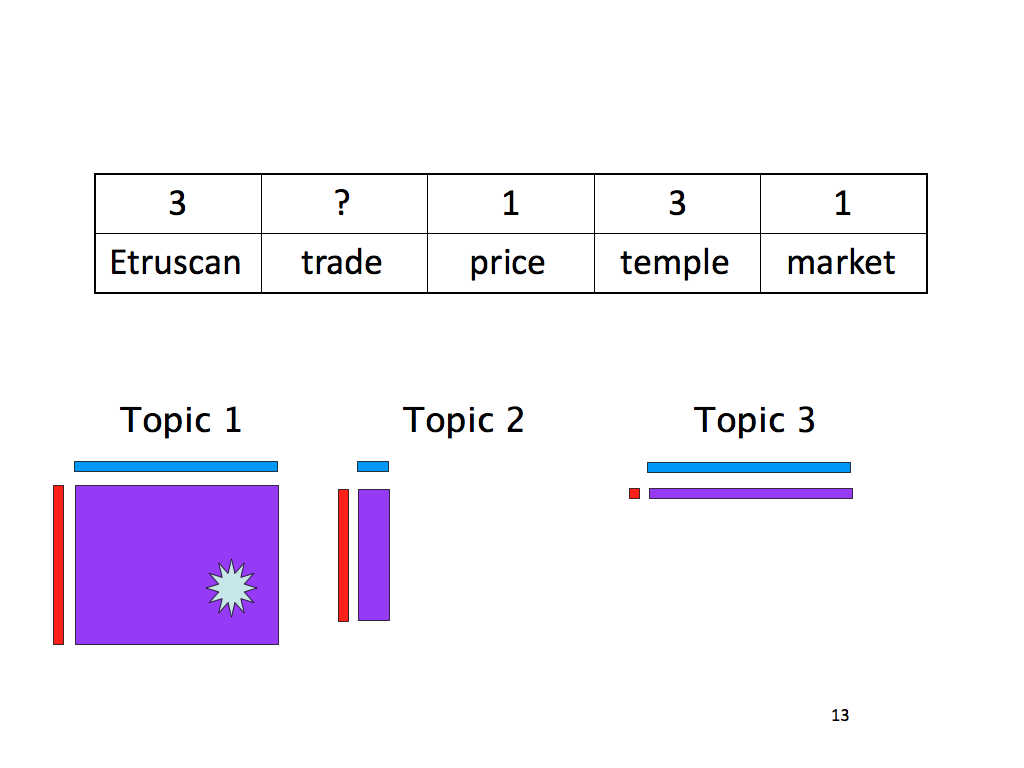
\includegraphics[width=\linewidth]{topic_models/mimno_013}}
\end{frame}

\begin{frame}
  \frametitle{Update counts}
    \only<1>{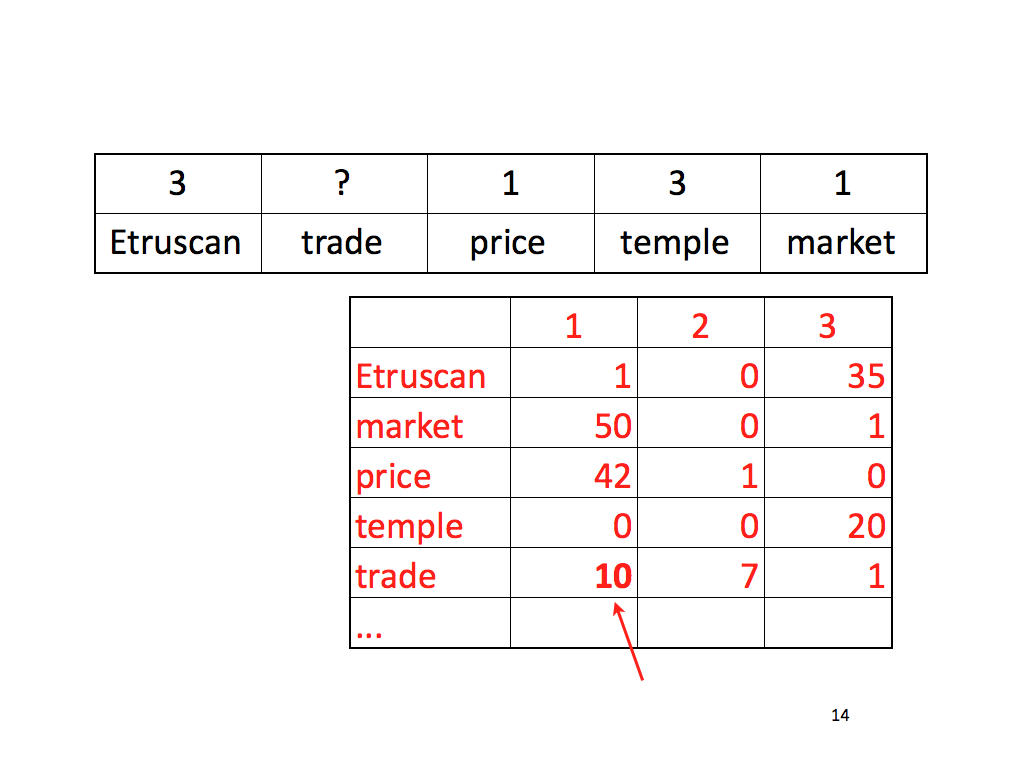
\includegraphics[width=\linewidth]{topic_models/mimno_014}}
    \only<2>{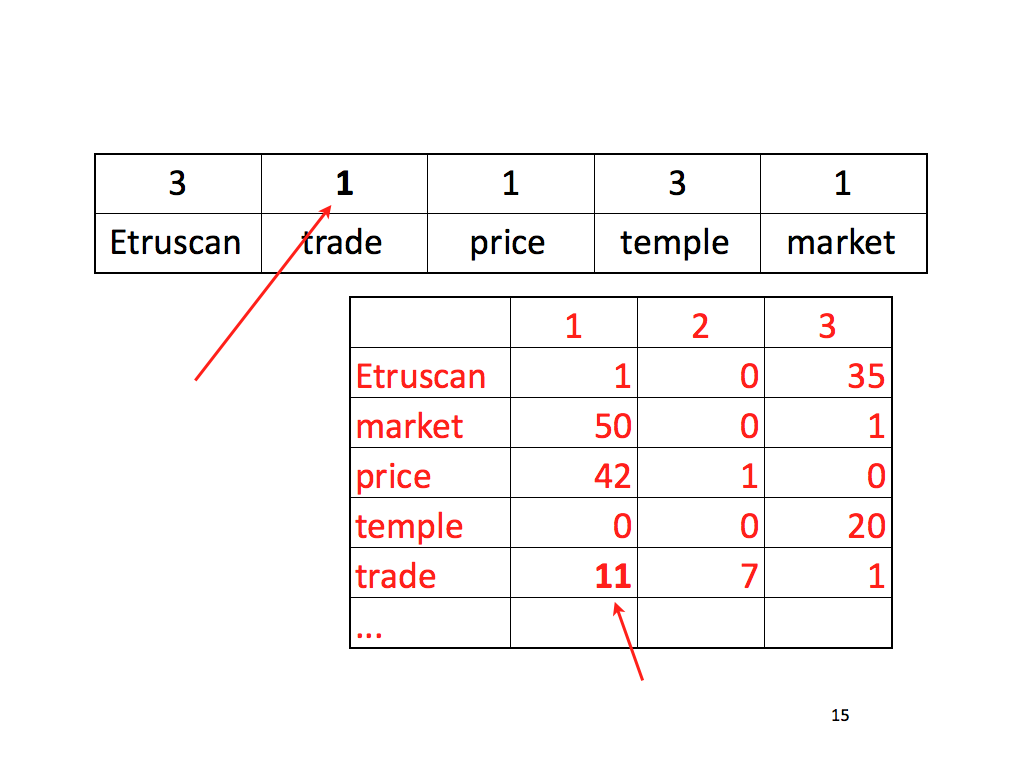
\includegraphics[width=\linewidth]{topic_models/mimno_015}}
    \only<3>{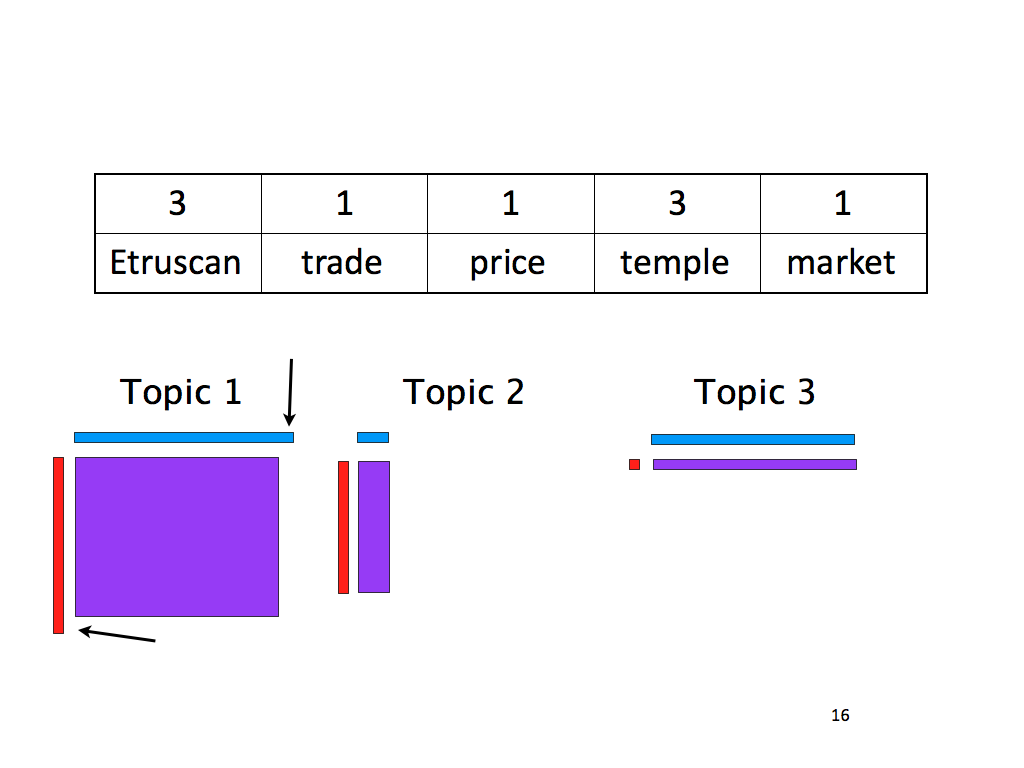
\includegraphics[width=\linewidth]{topic_models/mimno_016}}
\end{frame}


\begin{frame}
  \frametitle{Details: how to sample from a distribution}

\begin{center}
  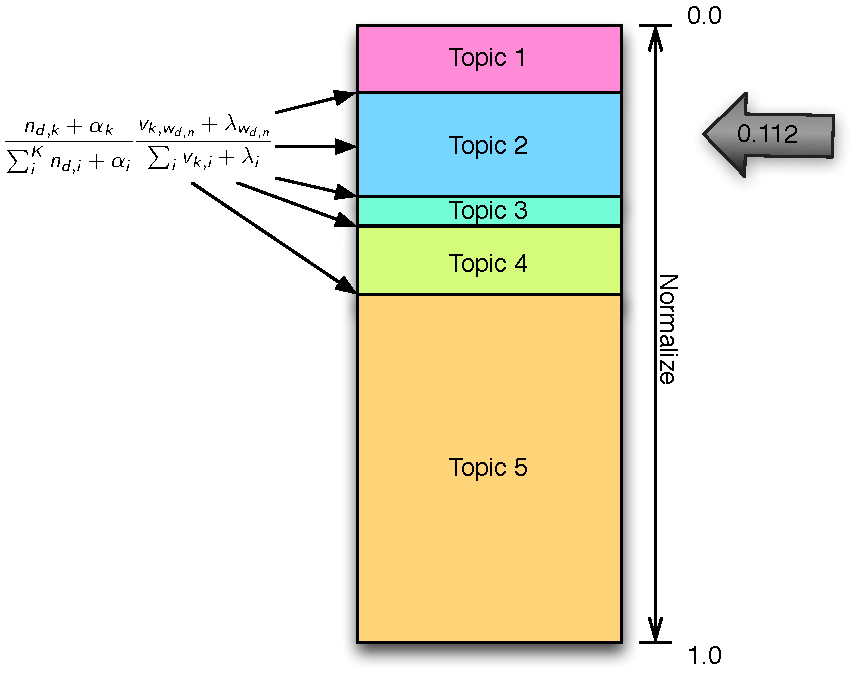
\includegraphics[width=.8\linewidth]{topic_models/sampling_from_distribution}
\end{center}
\end{frame}

\begin{frame}

\begin{block}{Algorithm}
\begin{enumerate}
\item For each iteration $i$:
\begin{enumerate}
\item For each document $d$ and word $n$ currently assigned to $z_{old}$:
\begin{enumerate}
\item Decrement $n_{d,z_{old}}$ and $v_{z_{old}, w_{d,n}}$
\item Sample $z_{new} = k$ with probability proportional to $\frac{n_{d, k} + \alpha_k}{ \sum_{i}^{K} { n_{d,i} + \alpha_i}} \frac{v_{k, w_{d,n}} + \lambda_{w_{d,n}}}{ \sum_{i} { v_{k,i} + \lambda_{i}}}$
\item Increment $n_{d,z_{new}}$ and $v_{z_{new}, w_{d,n}}$
\end{enumerate}
\end{enumerate}
\end{enumerate}
\end{block}

\end{frame}

\begin{frame}

\frametitle{Implementation}

\begin{block}{Algorithm}
\begin{enumerate}
\item For each iteration $i$:
\begin{enumerate}
\item For each document $d$ and word $n$ currently assigned to $z_{old}$:
\begin{enumerate}
\item Decrement $n_{d,z_{old}}$ and $v_{z_{old}, w_{d,n}}$
\item Sample $z_{new} = k$ with probability proportional to $\frac{n_{d, k} + \alpha_k}{ \sum_{i}^{K} { n_{d,i} + \alpha_i}} \frac{v_{k, w_{d,n}} + \lambda_{w_{d,n}}}{ \sum_{i} { v_{k,i} + \lambda_{i}}}$
\item Increment $n_{d,z_{new}}$ and $v_{z_{new}, w_{d,n}}$
\end{enumerate}
\end{enumerate}
\end{enumerate}
\end{block}

\end{frame}


\begin{frame}
\frametitle{Desiderata}
\begin{itemize}
\item Hyperparameters: Sample them too (slice sampling)
\item Initialization: Random
\item Sampling: Until likelihood converges
\item Lag / burn-in: Difference of opinion on this
\item Number of chains: Should do more than one
\end{itemize}
\end{frame}

\begin{frame}
	\frametitle{Available implementations}

	\begin{itemize}
		\item Mallet (http://mallet.cs.umass.edu)
		\item LDAC (http://www.cs.princeton.edu/~blei/lda-c)
		\item Topicmod (http://code.google.com/p/topicmod)
	\end{itemize}
\end{frame}